\documentclass[]{article}
%Fonts
\usepackage[utf8]{inputenc}
\usepackage[T1]{fontenc}
\usepackage{XCharter} 

\usepackage{graphicx}
\usepackage{booktabs}   
\usepackage[document]{ragged2e}
% Table
\usepackage{tabularx}
\usepackage{multirow}
% URL
\usepackage{hyperref}

%DOCUMENT MARGINS
\usepackage{geometry} 
\usepackage{graphicx,wrapfig,lipsum}

\geometry{
	paper=a4paper, % Paper size, change to letterpaper for US letter size
	top=2.5cm, % Top margin
	bottom=3cm, % Bottom margin
	left=2.5cm, % Left margin
	right=2.5cm, % Right margin
	headheight=14pt, % Header height
	footskip=1.5cm, % Space from the bottom margin to the baseline of the footer
	headsep=1.2cm, % Space from the top margin to the baseline of the header
	%showframe, % Uncomment to show how the type block is set on the page
}
% ----------------------------------------
\begin{document}
\newgeometry{top=5cm,bottom=0.1cm}
\begin{titlepage}
\begin{center}

    \textbf{\LARGE \vspace*{15pt}Indian Institute of Technology, Kanpur}
\end{center}
\begin{figure}[h]
\centering

\includegraphics[scale=0.7]{bluelog.jpg}
\end{figure}
    \begin{center}
    \textbf{\Large CS685A: Data Mining\\
        Mid-Term Project Report 2020\\}
\end{center}


\begin{center}
\vspace{1 cm}
\rule{\textwidth}{2pt}\linebreak
\Large
\textbf{Title: Analysis of number of child births and infant deaths in India}
\rule{\textwidth}{2pt}\\
\vspace{2.5 cm}
\Large
\textbf{Supervised By: Prof. Arnab Bhattacharya}\\
\vspace{2.5cm}
\normalsize{16 October 2020}
    
\end{center}
\end{titlepage}
\newpage

\restoregeometry
\begin{titlepage}
    \begin{center}
        \begin{center}
        \textbf{\Large Submitted By: Group 5}\\
        \end{center}
        
        \medskip
        
        \vspace{1cm}
        \rule{\textwidth}{2pt}
        \large{Lavlesh Mishra \hfill 19111048(lavleshm@iitk.ac.in)}\\
        \large{Kuldeep Kumar Solanki \hfill 19111045(kuldeeps@iitk.ac.in)}\\
        \large{Jaydeep Meda \hfill 19111039 (jaydeepm@iitk.ac.in)}\\
        \large{Aditya Jain \hfill 20111004 (adityaj20@iitk.ac.in)}\\
        \large{Rohit Singh \hfill 20111418 (kun20@iitk.ac.in)}\\
        \medskip
        \rule{\textwidth}{2pt}
    \end{center}
\end{titlepage}
\newpage
\tableofcontents
\newpage
\section{Abstract}
\justifying
This report narrates few main aspects of the project like, our approach for dataset preparation starting from methods used for data extraction to steps involved in data pre-processing. It also describes the work done till now, with expected results followed by ways to evaluate them.
        
\section{Broad Aims of the project}
To create a model that predicts the number of child births and infant deaths in a year for all district of India.

\section{Datasets}
\subsection{Performance of Key Health Management Indicators for each district in India}
        
This data is released by Ministry of Health under National Health Mission flagship program which seeks to provide effective healthcare to the rural population throughout the country.

\bigskip

Data set includes the key indicators which affects health of mother and child during pregnancy and at the time of delivery. Data also reports the number of children born and number on infant deaths in each district in a particular year. Data set is available for years 2008 to 2019.

\bigskip

Link: \url{https://www.nrhm-mis.nic.in/hmisreports/frmstandard_reports.aspx}
   
\subsection{Census Data 2001 and 2011}

The Census of India is conducted every 10 years Ministry of Home Affairs. The Census Data is available in public domain. The data is available at district level for total population, age, disability, education, migration, religion, and various other features.

\medskip

Link to Census 2001: \url{https://censusindia.gov.in/DigitalLibrary/TablesSeries2001.aspx}

\medskip

Link to Census 2011: \url{https://censusindia.gov.in/2011census/population_enumeration.html}
    
\section{Data Preparation}

\subsection{Pre-processing of HMIS data:}

The data of the Health Management Information System (HMIS) database was given in the form of excel files and in state wise manner for each financial year from 2008-09 to 2018-19. Initially, the dataset contained a lot of unnecessary information that we did not use.

\bigskip

We have filtered the dataset and selected the relevant attributes for the prediction of the number of births in a particular district in a particular year.

\subsection{Pre-processing of Census data:}
The data of census was given in form of excel files. We have manually pre-processed the excel file to extract the required data. The data was present for the year 2001 and 2011. So we have generated the data for the years 2002-2019, using the Compound Interest formula.
\begin{itemize}
\item The Growth Rate(r) is calculated using the 2001 data as Principal(p) and 2011 data as the final amount(p+i). Here i is the Interest.
\item Data is generated for the remaining years using calculated growth rate(r).
\end{itemize}
Correction of district and state names over the years for both the datasets. As new districts are introduced, or name of a district is changed over the years 2008 to 2019.

\newpage

\section{Work Done Till Now.}
\subsection {Pre-processing: }
As a test case we have applied the above pre-processing and different Machine Learning techniques for the Gujrat state.

\bigskip

The data from the year 2008 to 2017 is used to train the models and the testing was done for the year 2018. We have predicted the no. of births for the year 2018 district wise in Gujrat state. There are 26 districts in Gujrat state. Each district is given a district id from the numbers 0-25. 

\bigskip

The Features used in training the models from HIMS datasets are:
\begin{itemize}
\item Number having Hb level<11 (tested cases) 
\item Number having severe anaemia (Hb<7) treated at institution 
\item  Number of home deliveries attended by Non SBA trained (trained TB/Dai)
\item Number of C-section deliveries conducted at public facilities 
\item Number of C-section deliveries conducted at private facilities
\item Total Number of reported Still Births
\item Total Number of Abortions ( Spontaneous/ Induced) Reported
\item Total Number of MTPs ( Public) reported
\item Number of Vasectomies Conducted (Public + Pvt.)
\item Number of Tubectomies Conducted (Public + Pvt.)
\item Total Sterilisation Conducted
\item IUCD Insertions done (public facilities)
\item IUCD insertions done (pvt. facilities)
\item Oral Pills distributed
\item Condom pieces distributed
\item Adverse Events Following Immunisation (Others)
\item Number of Major Operations
\item Number of Minor Operations
\item Total Number of Infant Deaths reported
\end{itemize}

The Features used in training the models from census datasets are:
\begin{itemize}
\item Population Persons
\item Literate Persons
\item Main workers Persons
\item Marginal workers Persons
\item Non-workers Persons
\end{itemize}

\newpage
\subsection{Results Obtained}
The training and testing score using different Machine Learning Techniques:


\begin{table}[h]
    \centering
    \begin{tabular}{||c c c||}

\hline
Model Name&Training Score&Testing Score  \\[1ex]
 \hline \hline
Linear Regression&0.9670404857345802 &0.8150463694405432 \\[1ex]
 \hline
Ridge Regression&0.9670404857345805&0.8150463696084705\\[1ex]
\hline
Lasso Regression&0.966971710557302&0.8188446199470976\\[1ex]
\hline
Random Forest&0.9915817817676562&0.9441529668423073\\[1ex]
\hline

\end{tabular}
    \caption{Prediction Accuracy}
    
\end{table}

The Random Forest Regressor Model performs the best with training accuracy of  99.15\% and testing accuracy of 94.41\%. 


\subsection{Results Evaluation}
\textit{Figure 1.} is the graph for prediction of births in Gujrat state district wise for the year 2018. The 'Districts' axis in the graph is 'district id' and 'Births' axis is the 'no of births in the corresponding district'.

\begin{figure}[h]
\centering
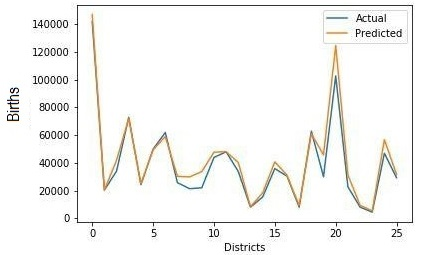
\includegraphics[scale=1]{graph.jpg}
\caption{Random Forest Prediction Graph}
\end{figure}

\bigskip

The most significant features as per the Random Forest Regressor:

\medskip

\begin{minipage}[t]{0.5\textwidth}
\begin{itemize}
\item Non-workers Persons
\item Population Persons
\item Literate Persons
\item Number of Tubectomies Conducted (Public + Pvt.)
\item Total Sterilisation Conducted
\end{itemize}
\end{minipage}
\begin{minipage}[t]{0.5\textwidth}
\begin{itemize}
\item Main workers Persons
\item Total Number of reported Still Births
\item Oral Pills distributed
\item Number having severe anaemia (Hb<7) treated at institution
\item IUCD Insertions done (public facilities)
\end{itemize}
\end{minipage}

\newpage

\section{Results to be obtained}
The results obtained are:
\begin{itemize}
\item Total no. of Child Birth for the Year 2020.
\item Total no. of Infant Deaths for the Year 2020.
\end{itemize}

\section{Evaluation of Results}
We will divide our datasets in two parts: Training set \& Test set. The data from the year 2008 to 2017 will be used as training set and the data for the year 2018 will be used as test set. Accuracy of the model developed will be evaluated based on this test set. \\

\section{Important Links and References}
\begin{itemize}
\item HMIS Database:\url{https://www.nrhm-mis.nic.in/hmisreports/frmstandard_reports.aspx}
\item Census Data 2001:\url{https://censusindia.gov.in/DigitalLibrary/TablesSeries2001.aspx}
\item Census Data 2011:\url{https://censusindia.gov.in/2011census/population_enumeration.html}
\item GitHub Link for the project: \url{https://github.com/kuldeeps5/DataMiningFinalProject}
\item Implementation of Lasso and Ridge Regression: \\\url{https://analyticsindiamag.com/hands-on-implementation-of-lasso-and-ridge-regression/}
\item Random Forest Regression: \url{https://www.geeksforgeeks.org/random-forest-regression-in-python/}
\end{itemize}

   


\end{document}

